\section{Theory}
\begin{frame}{What was known before!}
    
\end{frame}
\begin{frame}{Theory from Austria - What we understand!}
    \begin{bigidea}{Key Idea}
        Instead of using $B^\star$ and $D^\star$ and the wall picture $\Rightarrow$ the bath thermalizes the rotor!
    \end{bigidea}
    The Hamiltonian that describes the molecule in the centrifuge:
     \[
  \boxed{
    \hat{H}_{\mathrm{lab}}(t) =
  BJ^2 + \hat{R}(t)^\dagger
  \hat{V}_{\mathrm{drive}}\hat{R}(t) 
  }
  \qquad \text{with}\quad
  \hat{R}(t) = e^{i\Omega t \hat{L}_{Z}}
\]
\textbf{1. Assumption:} $t_{\mathrm{bath}} << \Omega^{-1}$ and $\Omega$ is const. for each time step
\begin{itemize}
    \item the bath is fast compared to rotation
    \begin{itemize}
        \item each time step can be treated independently
    \end{itemize}
\end{itemize}
\vspace{0.1cm}
under the assumption the Lindblad equation becomes a simple Master's equation:
\[
\partial_t \rho_{\mathrm{lab}}(t)
=
i\left[\hat{H}_{\mathrm{lab}}(t), \rho_{\mathrm{lab}}(t)\right]
-
\frac{
\rho_{\mathrm{lab}}(t)
-
\frac{1}{Z}\exp\!\left[\hat{H}_{\mathrm{lab}}(t)/T\right]
}{
\tau_{\mathrm{relax}}
}
\]
    
\end{frame}

\begin{frame}{Theory from Austria - What we understand!}
   
In the rotating frame $\hat{H}$ is time-independent
        \[
  \boxed{
    \hat{H}_{\mathrm{rot}} =
  BJ^2 + \hat{V}_{\mathrm{drive}} - \Omega \hat{L}_Z
  }
\]
With $\rho_0$ being the density matrix of the non-rotating drive
\[
\rho_0
=
\frac{1}{Z}
\exp\!\left[
\left(
BJ^2 + \hat{V}_{\mathrm{drive}}
\right)/T
\right]
\]
The Master's equation simplifies to:
\[
\partial_t \rho_{\mathrm{rot}}
=
i\left[\hat{H}_{\mathrm{rot}}, \rho_{\mathrm{rot}}\right]
-
\frac{
\rho_{\mathrm{rot}} - \rho_0
}{
\tau_{\mathrm{relax}}
}
\]
\end{frame}

\begin{frame}{Theory from Austria - What we understand!}
\textbf{2. Assumption:} $\tau_{\mathrm{relax}} << t_{\mathrm{experiment}}$ 
\begin{itemize}
    \item relaxation time must be smaller than the time on which the experimental situation change noticeably
    \begin{itemize}
        \item steady state matrix with no dynamical effects
    \end{itemize}
\end{itemize}
\[
\partial_t \rho_{\mathrm{rot}} = 0 =
-\frac{i}{\hbar}
\left[
\hat{H}_{\mathrm{rot}},\hat{\rho}_{\mathrm{ss}}
\right]
-
\frac{
\hat{\rho}_{\mathrm{ss}}-\hat{\rho}_0
}{
\tau_{\mathrm{relax}}
}
\]
Next step is to find the eigenbasis of $\hat{H}_{\mathrm{rot}}$
\[
\hat{H}_{\mathrm{rot}} | a \rangle = E_{a} | a \rangle
\]
\[
\rightarrow \qquad
\boxed{\left\langle a \middle| \hat{\rho}_{\mathrm{ss}} \middle| b \right\rangle
=
\frac{
\left\langle a \middle| \hat{\rho}_0 \middle| b \right\rangle
}{
1+i\tau_{\mathrm{relax}}
\left(E_a-E_b\right)
}}
\]
\end{frame}
\begin{frame}{Theory from Austria - The picture behind the formulas}
\[\left|\rho^{\mathrm{ss}}_{ab}\right|
=
\frac{
\left|\rho^0_{ab}\right|
}{
\sqrt{
1+
\tau_{\mathrm{relax}}^2
\left(E_a-E_b\right)^2
}
}
\qquad
\hat{H}_{\mathrm{rot}} =
  BJ^2 + \hat{V}_{\mathrm{drive}} - \Omega \hat{L}_Z
\]
\vspace{0.05cm}
\noindent\rule{\linewidth}{0.5pt}
\vspace{0.05cm}
To draw an easier picture in our heads let's assume $| a \rangle$ are more or less similar to the spherical harmonics: 
\twocol{\[
\hat{\rho}_0
=
\begin{array}{c}
\begin{array}{cccc}
Y_0^0 & Y_1^{-1} & Y_1^0 & Y_1^1
\end{array}
\\
\left(
\begin{array}{cccc}
0.40      & \rho_{12} & \rho_{13} & \rho_{14} \\
\rho_{21} & 0.25      & \rho_{23} & \rho_{24} \\
\rho_{31} & \rho_{32} & 0.20      & \rho_{34} \\
\rho_{41} & \rho_{42} & \rho_{43} & 0.15
\end{array}
\right)
\end{array}
\begin{array}{l}
Y_0^0 \\
Y_1^{-1} \\
Y_1^0 \\
Y_1^1
\end{array}
\]}{
    \vspace{0.9cm}
    \begin{itemize}
        \item diagonal elements correspond to the probability of the state
        \item off diagonal elements describe \textbf{coherence}
    \end{itemize}
}
    
\end{frame}
\begin{frame}{Theory from Austria - What we understand!}
    \begin{bigidea}{What does that mean for the oscillations?}
        \begin{itemize}
            \item \textbf{Fast relaxation and low $\Omega$:} the density matrix of the non-rotating drive is recovered as the bath thermalizes at each direction
            \begin{itemize}
                \item strong signal in $cos^2(\theta)$
            \end{itemize}
            \item \textbf{Slow relaxation and large $\Omega$:} $\rho_{\mathrm{ss}}$ is more $\hat{H}_{\mathrm{rot}}$ like $\rightarrow$ coherence is lost
            \begin{itemize}
                \item lower signal in $cos^2(\theta)$
            \end{itemize}
        \end{itemize}
    \end{bigidea}
\end{frame}
\begin{frame}{Comparing Theory and Experiment}
    \begin{figure}
    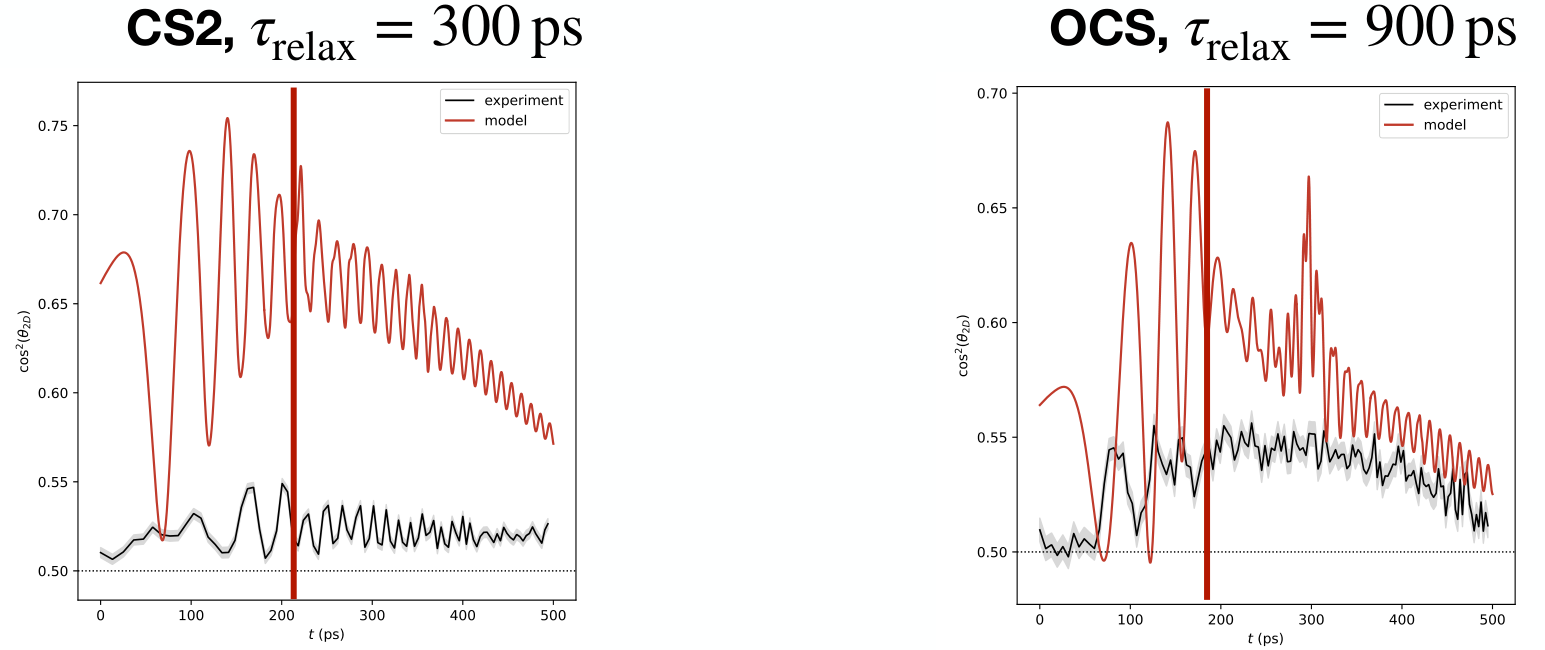
\includegraphics[width=\linewidth]{figures/theory_exp_comparison.png}
  \end{figure}
\end{frame}